\documentclass[9pt,a4paper,twoside]{tau}
\usepackage[english]{babel}
\usepackage{tauenvs}

%----------------------------------------------------------
% TITLE
%----------------------------------------------------------

\title{CVML-Pose: Convolutional VAE Based Multi-Level}
%----------------------------------------------------------

\author[a,1]{JIANYU ZHAO}
\author[b,2]{EDWARD SANDERSON}
\author[c,3]{ BOGDAN J. MATUSZEWSKI}

%----------------------------------------------------------

\affil[a]{Graduate Student Member, IEEE}
\affil[b]{Member, IEEE}
\affil[c]{Member, IEEE}

\professor{Computer Vision and Machine Learning (CVML) Group, University of Central Lancashire, PR1 2HE Preston, U.K}

%----------------------------------------------------------
% FOOTER INFORMATION
%----------------------------------------------------------

\institution{College name}
\ftitle{\LaTeX\ Template}
\date{April 10, 2024}
\etal{Author last name et al.}
\course{Creative Commons CC BY 4.0}
%----------------------------------------------------------
% FOOTER INFORMATION
%----------------------------------------------------------
\ftitle{\LaTeX\ CVML-Pose: Convolutional VAE Based Multi-Level}
%----------------------------------------------------------

\begin{document}	
	\maketitle
	\thispagestyle{firststyle}
	\tableofcontents
        \tableofcontents

\section{Introduction}

    \taustart{M}ost state-of-the-art methods, for 3D pose estimation typically require object’s 3D model or 2D-3D correspondence information. Approaches that rely on 2D-3D correspondence estimate pixel-wise dense correspondence or matching between a number of sparse keypoints. Subsequently, these approaches estimate pose through various Perspective-n-Point (PnP) algorithms.
    
\section{Network for Object 3D Pose Estimation }
\begin{figure}[H]
                \centering
                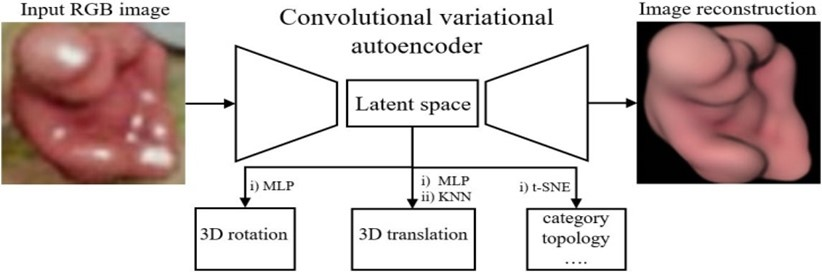
\includegraphics[width=0.8\columnwidth]{Figures/Picture1.jpg}
                \caption{CVML-Pose pipeline. During training, the convolutional variational autoencoder captures object’s latent representation in its latent space that is further interpreted to object 3D pose, category, and topology using MLPs, KNN, and t-SNE.}
                \label{fig:figure}
            \end{figure}
\begin{figure}[H]
                \centering
                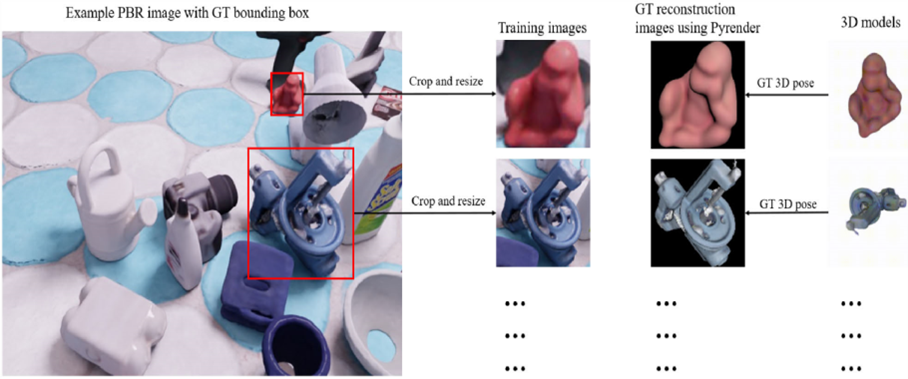
\includegraphics[width=0.8\columnwidth]{Figures/Picture2.png}
                \caption{Example Data preprocessing based on the LineMod  objects. GT stands for ground truth, and the ground truth information.}
                \label{fig:figure}
            \end{figure}
        Besides, Pyrender is used to additionally synthesize ground truth (GT) reconstruction images xˆ with a clean background based on the ground truth 3D pose and camera intrinsic parameters provided by the LineMod PBR database. Fig. 2 illustrates how the LineMod PBR images and ground truth reconstruction images are prepared. Please notice that the ground truth reconstruction images xˆ are different from the input images x of the object of interest, as shown , xˆi shows a complete object without any background or occlusions, which could be possibly present in the original input image $x_i.$
        
        With the assumed distribution $p_\Theta$(x|z), $q_\phi$(z|x), and p(z), the KL divergence $D_{KL}$($q_\Phi$(z|$x_i$)||p(z)) has a close form and the ELBO in Eq.\ref{eq:ELBO} can be estimated using:
	\begin{equation} \label{eq:ELBO}
            ELBO \cong -c \sum_{i=1}^{m} \left( ||x_i - x_i||^{'2} - \alpha \sum_{(j=1)}^{n} \left(1 + \log(\sigma_{ij}^2) - \mu_{ij}^2 - \sigma_{ij}^2 \right) \right)
        \end{equation}
        where c is a positive constant,
        \begin{itemize}
        \item $x_i$ is the input data, 
        \item $x_i'$ is the output reconstruction, 
        \item $x_i' = x_\theta(z(x_i'))$, 
        \item $\mu_{ij}$ refers to the j element of the vector $\mu_{i}$, 
        \item $\sigma_{ij}^2$ refers to the j element of the vector \item $\sigma_{i}^2$, 
        \item m represents the number of data points in the training set, and n refers to the dimensionality of the latent space.
        \end{itemize}
Hence, the contributions of this work could be outlined as follows:
    \begin{itemize}
	\item[-] A thorough taxonomy of the existing works is conducted with reference to various aspects, such as the methodology deployed to design the proposed models, types of image data that could be processed by the subject technology, and their application scenarios.
	\item[-] Public datasets deployed to validate the proposed models on 3D point cloud data are discussed and compared with regard to different parameters.
	\item[-] Several comparisons of the most significant works identified in the state-of-the-art have been conducted to demonstrate their performance across multiple datasets and metrics.
	\item[-] Current challenges and issues that remained unresolved have been targeted. Insights about future directions and trends have been discussed along with their potential impact on research and development in the near and distant future.
    \end{itemize}
This suggests a two-step approach:
\begin{enumerate}
    \item Find a set of primary matches using the conventional forward matching scheme, and designate as preferred matches a subset of them with low distance ratios (and hence relatively higher confidence).
    \item Augment the set of primary matches by performing a prioritized inverse matching starting from the preferred matches as the model points to search for in the images.
\end{enumerate}
    	
The final pose estimation is carried out on the augmented set of matches.
If the model point isn’t observed, the corresponding points within the distance threshold dth in partial view point cloud will not appear. At last, the observability of the model point p is calculated according to (\ref{eq:Obs}).

    \begin{equation} \label{eq:Obs}
        Obs(p) =\frac{1}{K} \sum_{k=1}^{K-1} \delta(p, o_k)
    \end{equation}
Here, K represents the number of viewpoints. $o_k$ represents the direction of the viewpoint vector, and the function  $\delta$ returns "1" when the model point p is observed.
            
    \begin{table}[H]
        \centering
        \caption{Average precision of the ADD(S) metric evaluated on the LineMod objects. The glue and eggbox are considered as symmetric objects, bowl and cup are not included due to the reported problems with their 3D models in the LineMod dataset, leading to inaccurate computations of the ADD(S) metric. Since Multi-Path, EPOS, and CosyPose do not provide results on the LineMod test data, we only report their LineMod-Occlusion results in Table 2}
    \label{tab:table}
        \begin{tabular}{lllllllll}
            & \multicolumn{3}{l}{Latent repsresantatyion based methods}\\
Objects     & CVML-18            & AAE              & AAE-ICP           & SS6D6         \\
Ape         & 26.64              & 4.18             & 24.35             & 2.6           \\
benchvise   & 52.47              & 22.85            & 89.13             & 15.1          \\
cam         & 25.68              & 32.91            & 82.10             & 6.1           \\
can         & 50.05              & 37.03            & 70.82             & 27.3          \\
driller     & 47.81              & 24.81            & 44.87             & 12.0          \\
duck        & 24.44              & 5.86             & 54.63             & 1.3           \\
eggbox      & 77.41              & 81.00            & 96.62             & 2.8           \\
glue        & 55.08              & 46.17            & 94.18             & 3.4           \\
holepuncher & 21.05              & 18.20            & 51.25             & 3.1           \\
iron        & 54.85              & 35.05            & 77.86             & 14.6          \\
lamp        & 54.13              & 61.15            & 86.31             & 11.4          \\
phone       & 28.50              & 36.27            & 86.24             & 9.7           \\
AP(ADD(S))  & 42.64              & 32.63            & 71.58             & 9.1           
\end{tabular}
    \end{table}
    \begin{table}[H]
        \centering
        \caption{Average recall rate of the MSSD and the MSPD metrics based on the BOP version of the LineMod-Occlusion data. Our results are based on the CVML-18 network. Results of other approaches are from the BOP challenge leaderboard, results for individual object are not reported here since the challenge only provides the results for all objects. Please note CVML-18, CosyPose, Pix2Pose, CDPN, CDPNv2, EPOS and PVNet all use the LineMod PBR images, CDPNv2 refers to the extended version of CDPN, CosyPose uses object’s 3D model during training for iterative refinement.}
    \label{tab:table}

\begin{tabular}{lllllll}
       & \multicolumn{2}{c}{Latent representation based methods} & \multicolumn{2}{c}{Direct methods}\\
Metric & CVML-18                & AAE                & SSD6D          & Cosy\\
ARMSSD & 0.338                  & 0.095              & 0.083          & 0.606\\
ARMSPD & 0.706                  & 0.254              & 0.285          & 0.812           
\end{tabular}      
    \end{table}

The final pose estimation is carried out on the augmented set of matches.
\begin{equation} \label{eq:dis}
            x= \frac{-b \pm \sqrt{b^2 - 4ac}}{2a}
        \end{equation}
where b and c denote the focal lengths,
\begin{itemize}
        \item (a, b)-principal point.
        \end{itemize}
%----------------------------------------------------------

\end{document}